	
	
\selectlanguage{french} %ou english
\renewcommand{\tablename}{Tableau}
\renewcommand{\figurename}{Figure}
\chapter{Informations supplémentaires pour le chapitre~\ref{chapter_5}}
\label{annexeChap5}
	

  
\section{Un modèle d'interactions plante -- nématodes avec résistance tardive}
\label{diff_mod}


\begin{wrapfigure}[6]{L}{0.2\textwidth}
  \vspace{-\baselineskip}
  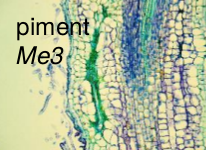
\includegraphics[width=\linewidth]{pimentMe3.png}
\end{wrapfigure}
\noindent
Dans la \autoref{sec:introduction-virulents} et le \autoref{chapter2} \eqref{sys1}, nous avons présenté un modèle d'interaction plante-nématodes, dans lequel les plantes peuvent être porteuses d'un gène \textbf{résistance précoce}, tel que \textit{Mi-1} chez la tomate ou \textit{Me3} chez le piment. Quand un nématode avirulent sous sa forme libre J2  tente de pénétrer dans la racine,  il est piégé au niveau du cortex racinaire de la plante dès le premier jour.
\bigskip

\begin{wrapfigure}[6]{L}{0.2\textwidth}
  \vspace{-\baselineskip}
  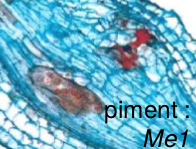
\includegraphics[width=\linewidth]{pimentMe1.png}
\end{wrapfigure}
\noindent
Il existe également des gènes de \textbf{résistance tardive}, tels que \emph{Me1} chez le piment. Lorsqu'elle porte ce type de gène, la réponse de la  plante se produit plus tard, quelques jours après que le nématode a pénétré et migré dans la racine. La plante inhibe le développement des cellules géantes qui servent de site nourricier au nématode, bloquant ainsi son développement.

Dans le chapitre de conclusion, en \autoref{sec:compR-resistance-precoce-tardive}, nous comparons les deux types de résistance. Nous présentons ci-dessous le modèle avec résistance tardive qui a servi à obtenir nos résultats.

\paragraph{Interactions plante sensible --  nématodes avirulents}

Dans ce modèle, les interactions entre plantes sensibles (exposant $^S$) et nématodes avirulents (indice $_a$) sont les mêmes que dans le modèle précédent à la \autoref{sec:nos-hypotheses}  et le \autoref{chapter2} \eqref{eq:planteS-nemavir} :
\begin{equation*}
  \left\{
    \begin{aligned}
      \dot{P_a} &=- \beta H^S P_a - \eta P_a + r I_a,\\
      \dot{H^S} &= \mu x f(H^S,E_a,I_a)- \epsilon \beta P_a H^S,\\
      \dot{E_a} &= \epsilon \beta P_a H^S- \lambda E_a,\\
      \dot{I_a} &= \lambda E_a - \alpha I_a,
    \end{aligned}
  \right.
\end{equation*}
avec $f(H^S,E_a,I_a)= e^{-k \pi}$ et $\pi=\frac{E_a +I_a}{H^S+E_a+I_a}$.

$\mu x f$ représente toujours la croissance de la plante, qui est freinée par la prévalence $\pi$ des unités de racines infectées. $\beta$ est le taux de contamination des racines saines et sensibles $H^S$ par des nématodes avirulents sous forme libre $P_a$. $\epsilon$ est le taux de conversion entre unité de racine et densité de nématodes ($\epsilon=1$). Le nématode $E_a$ établit son site nourricier dans la racine, puis au bout d'un temps $1/\lambda$ se transforme en femelle mature $I_a$ qui se reproduit à un taux $r$. $\eta$ et $\alpha$ sont les taux de mortalité des nématodes.

\paragraph{Interactions plante sensible --   nématodes avirulents et virulents}

L'introduction de nématodes virulents (indice $_v$) dans le modèle à résistance tardive est peu différente de \eqref{eq:mod-sensible} : 
\begin{equation}
  \left\{
    \begin{aligned}
      \dot{P_a} &=- \beta H^S P_a - \eta P_a + (1-\delta) r I_a,&\\
      \dot{P_v} &=- \beta H^S P_v - \eta P_v + \delta r I_a + (1-w_{r}) r I_v,\\
      \dot{H^S} &= \mu x f(H^S,E_a,E_v,I_v,I_a) - \epsilon \beta H^S (P_a + P_v),\\
      \dot{E_a} &= \epsilon \beta H^S P_a - \lambda E_a,\\
      \dot{E_v} &= \epsilon \beta H^S P_v - \lambda E_v,\\
      \dot{I_a} &= \lambda E_a - \alpha I_a,\\
      \dot{I_v} &= (1-\textcolor{navyblue}{w_{\lambda}}) \lambda E_v -\alpha I_v,
    \end{aligned}
  \right.
  \label{eq:planteS-nemav}
\end{equation}
avec $f(H^S,E_a,E_v,I_a,I_v)= e^{-k \pi}$ et $\pi=\frac{E_a+E_v+I_a+I_v}{H^S+E_a+E_v+I_a+I_v}$.

$\delta$ représente toujours la fraction de nématodes virulents issus de nématodes avirulents et $w_r$ le coût de fitness sur la reproduction. En revanche, le coût de fitness sur l'infection $w_\beta$, qui affecte le taux d'infection $\beta$ dans le modèle à résistance précoce, est remplacé ici par un coût de fitness $\textcolor{navyblue}{w_\lambda}$, qui intervient plus tardivement dans la racine. 

\paragraph{Interactions plante résistante --  nématodes avirulents et virulents}

Sur une plante résistante, les nématodes virulents ont le même développement que sur une plante sensible. Ce n'est pas le cas pour les nématodes avirulents. Leurs interactions avec une plante résistante diffèrent notablement selon que la résistance est précoce ou tardive. Dans ce second cas, les nématodes avirulents sous forme libre $P_a$ peuvent pénétrer dans la racine avec le taux d'infection $\beta$ utilisé pour les plantes sensibles, ce qui n'est pas le cas dans le modèle avec résistance précoce ($\epsilon_a^R=0$) pour la résistance précoce, alors que $\epsilon_a^R=\epsilon=1$ pour la résistance tardive). Cependant, au bout d'un temps assez court $\textcolor{navyblue}{1/\sigma}$ (2 jours environ), la plante bloque leur développement.

Nous supposons dans ce modèle qu'une attaque par un nématode avirulent déclenche les défenses de la plante et prévient ainsi localement toute autre attaque par un nématode. Le site nourricier initié par le nématode $E_a$ n'est alors plus disponible pour les autres nématodes. Il passe alors dans un état $\textcolor{navyblue}{G}$ \og immunisé \fg{}. Comme les défenses de la plante provoquent une nécrose au niveau du site nourricier, on suppose que seule une fraction $\textcolor{navyblue}{\psi}$ redevient de la racine saine (fonctionnelle) et immunisée $G$.

Le modèle ainsi obtenu diffère notablement du modèle \eqref{eq:ResistanceP-nemavir-nemvir} 
 avec résistance précoce (\autoref{fig:resistance_tardive}a). Il est décrit dans la \autoref{fig:resistance_tardive}b et s'écrit comme suit :

\begin{figure}[h]
   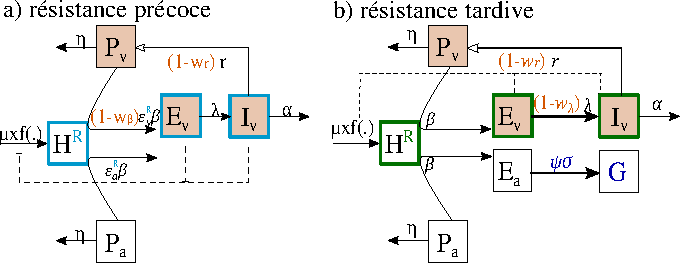
\includegraphics[width=1.1\linewidth]{mod_resistance-precoce-tardive.pdf}
  \caption[(a)  Schéma du modèle d'interactions plante avec résistance tardive -- nématodes]{Schéma du modèle d'interactions ~\eqref{eq:ResistanceP-nemavir-nemvir} entre une plante \textbf{avec résistance précoce} et des nématodes avirulents (indice $_a$) et virulents (indice $_v$).  (b)  Schéma du modèle d'interactions plante avec résistance tardive -- nématodesSchéma du modèle d'interactions ~\eqref{eq:resistance-tardive} entre \textbf{une plante avec résistance tardive} et des nématodes avirulents (indice $_a$) et virulents (indice $_v$).}
  \label{fig:resistance_tardive}
\end{figure}

\begin{equation}
  \left\{
    \begin{aligned}
      \dot{P_a} &=- \beta H^R P_a - \eta P_a,\\
      \dot{P_v} &=- \beta H^R P_v - \eta P_v  + (1-w_{r}) r I_v,\\
      \dot{H^R} &= \mu x f(H^R,E_a,E_v,I_v) - \epsilon \beta H^R (P_a + P_v),\\
      \dot{E_a} &= \textcolor{navyblue}{\epsilon} \beta  H^R P_a - \textcolor{navyblue}{\sigma} E_a,\\
      \dot{E_v} &=  \epsilon \beta H^R P_v - \lambda E_v,\\
      \dot{I_v} &= (1-\textcolor{navyblue}{w_{\lambda}}) \lambda E_v -\alpha I_v,\\
      \dot{\textcolor{navyblue}{G}} & \textcolor{navyblue}{= \psi \sigma E_a},
    \end{aligned}
  \right.
  \label{eq:resistance-tardive}
\end{equation}
avec $f(H^R,E_a,E_v,I_v)= e^{-k \pi}$ et $\pi=\frac{E_a+E_v+I_v}{H^R+E_a+E_v+I_v+G}$.
 
	
\paragraph{Modèle général : résistance tardive avec immunité}

Le modèle général s'écrit alors ainsi, pour une plante sensible ($X=S$ et $\textcolor{navyblue}{\xi^S_a=1}$) ou résistante ($X=R$ et $\textcolor{navyblue}{\xi^R_a=0}$) :
\begin{equation}
  \left\{
    \begin{aligned}
      \dot{P_a} &=- \beta H^X P_a - \eta P_a + (1-\delta) r I_a,\\
      \dot{P_v} &=- \beta H^X P_v - \eta P_v + \delta r I_a + (1-w_{r}) r I_v,\\
      \dot{H^X} &= \mu x f(H^X,E_a,E_v,I_v,I_a) - \epsilon \beta H^X (P_a +  P_v),\\
      \dot{E_a} &= \textcolor{navyblue}{\epsilon} \beta H^X P_a - \textcolor{navyblue}{(1-\xi^X_a) \sigma}  E_a - \textcolor{navyblue}{\xi^X_a} \lambda E_a,\\
      \dot{E_v} &=  \epsilon \beta H^X P_v - \lambda E_v,\\
      \dot{I_a} &= \textcolor{navyblue}{\xi^X_a} \lambda E_a - \alpha I_a ,\\
      \dot{I_v} & = (1-\textcolor{navyblue}{w_{\lambda}}) \lambda E_v - \alpha I_v,\\
      \dot{\textcolor{navyblue}{G}} & \textcolor{navyblue}{= (1- \xi^X_a) \psi \sigma E_a},
    \end{aligned}
  \right.
  \label{RT_im}
\end{equation}
avec $f(H^X,E_a,E_v,I_a,I_v)= e^{-k \pi}$ et $\pi= \frac{E_a+E_v+I_a+I_v}{H^X+E_a+E_v+I_a+I_v+G}$.
	

À la fin de chaque saison, les plantes sont arrachées. Au début de la saison suivante, on suppose que les nouvelles plantes sont saines avec la même densité qu'au temps initial. Les nématodes présents dans le sol sous forme libre correspondent à une fraction $\varphi$ des nématodes présents à la fin de la saison précédente, comme pour le modèle avec résistance précoce, décrit en \eqref{eq:intersaison-nemavir-nemvir}.

\paragraph{Paramètres}

Les conditions initiales et les valeurs des paramètres utilisées sont les mêmes que celles du modèle avec résistance précoce présenté en \autoref{table1}, à l'exception des paramètres spécifiques présentés en  \autoref{tab:parametresRtardive} et de la condition initiale pour les racines immunisées $G(0)=0$.



\begin{table}[ht]
  \small
  \caption{Paramètres spécifiques du modèle de résistance tardive}
  \begin{tabular}{@{}l@{ }l@{ }l@{ }l@{ }l@{ }l@{}}
    \hline
    Symbole & Description                      & Valeur(s) & & Unité & Référence.\\
    \hline
    $\psi$  & Fraction de racine saine non nécrosée & $0,95$ & $(0,85;0,95;1)$ & --& -- \\
    $\sigma$ & Taux de passage entre $E_a$ à $G$ & $0,5$ &  & jour$^{-1}$ & \citet{Pegard2005} \\
    $w_\lambda$ & Coût de virulence sur l'infection  & $0,09$ &  & -- & -- \\    
    \hline
  \end{tabular}
    \label{tab:parametresRtardive}
  \par\medskip\footnotesize
 Les autres paramètres du modèle de résistance tardive et leur valeur sont les mêmes que les paramètres de référence du modèle de résistance précoce décrit dans le~\autoref{table1}.
\end{table}


\section{Un modèle avec réservoir de plantes sensibles non cultivées}

Dans le chapitre de conclusion, en~\ref{sec:compR-resistance-precoce-tardive}~\autoref{sec:plante-reservoir}, nous comparons plus particulièrement la durabilité des deux types de résistance lorsque l'on déploie uniquement des plantes résistantes. Comme les nématodes avirulents ne peuvent pas se reproduire sur les plantes résistantes, nous avons introduit un « réservoir » de plantes sensibles correspondant à des plantes sauvages, adventices ou à des débris de racines, présents toute l’année, mais ne présentant pas d’intérêt agronomique.

\paragraph{Modèle avec résistance tardive}

Pour le modèle avec résistance tardive, le réservoir se comporte comme la plante sensible décrite par~\eqref{eq:planteS-nemav}, mis à part la croissance des racines saines $S$. On suppose également que la croissance linéaire, mais  avec un taux $vx$ sans impact de l'infection, et on ajoute un terme de mortalité des racines avec un taux $\omega$. En notant $E'_a$ et $E'_v$ les racines occupées du réservoir par des nématodes respectivement avirulents et virulents en train d'initier leur site nourricier,  $I'_a$ et $I'_v$ les racines occupées par des nématodes matures, $P_a$ et $P_v$ représentant toujours les densités de nématodes sou forme libre dans le sol, on obtient le modèle suivant pour le réservoir :
\begin{equation}
  \left\{
    \begin{aligned}
      \dot{P_a} & =- \beta S P_a - \eta P_a + (1-\delta) r  I'_a,\\
      \dot{P_v} & =- \beta S P_v - \eta P_v + \delta r  I'_a + (1-w_{r}) r I'_v,\\
      \dot{S} &= v x - \epsilon \beta S (P_a + P_v) - \omega S,\\
      \dot{E'_a} &= \epsilon \beta S P_a - \lambda  E'_a,\\
      \dot{E'_v} &= \epsilon \beta S P_v - \lambda E'_v,\\
      \dot{I'_a} & = \lambda E_a' - \alpha I'_a,\\
      \dot{I'_v} & = (1-w_{\lambda}) \lambda E'_v - \alpha I'_v.
    \end{aligned}
  \right.
  \label{eq:reservoir0}
\end{equation}

  
La densité de racines saines de la plante réservoir à l'équilibre sans nématodes est :  
\begin{equation}
  S_{eq} = \dfrac{vx}{\omega}.
  \label{eq:Seq}
\end{equation}
On utilise cette quantité pour mesurer la taille du réservoir.

Pendant l'intersaison, on considère que la dynamique du réservoir est négligeable (pas de croissance, pas d'attaques de nématodes). En notant $T$ la durée d'une année et $\tau$ la durée d'une saison, la densité de racine saine $S$ en début de chaque saison est calculée de la manière suivante : 

	
\begin{equation}
	\left\{
		\begin{aligned}
		S((n+1)T)    &=S(nT+\tau),\\    
		E'_a ((n+1)T) &= 0,\\
		I'_v ((n+1)T) &= 0.
		\end{aligned}
	\right.
\label{eq:intersaison-plante-reservoir}
\end{equation}


Si l'on couple le modèle du réservoir ci-dessus avec le modèle d'interactions plantes-nématodes avec résistance tardive~\eqref{RT_im}, on obtient le modèle suivant :
\begin{equation}
  \left\{
    \begin{aligned}
      \dot{P_a} &= - \beta (H^X + S) P_a - \eta P_a + (1-\delta) r (I_a + I'_a),\\
      \dot{P_v} &= - \beta (H^X + S) P_v - \eta P_v + \delta r (I_a + I'_a) + (1-w_{r}) r (I_v + I'_v),\\
      \dot{H^X} &= \mu x f(H^X,E_a,E_v,I_a,I_v) - \epsilon \beta  H^X (P_a + P_v),\\
      \dot{E_a} &= \epsilon \beta H^X  P_a - (1-\xi^X_a) \sigma  E_a - \xi^X_a \lambda E_a,\\
      \dot{E_v} &= \epsilon \beta H^X P_v - \lambda E_v,\\
      \dot{I_a} &= \xi^X_a \lambda E_a  - \alpha I_a ,\\
      \dot{I_v} &= (1-w_{\lambda}) \lambda E_v - \alpha I_v,\\
      \dot{G} &= (1- \xi^X_a) \psi \sigma  E_a,\\
      \dot{S} &= v x - \epsilon \beta S (P_a + P_v) - \omega S,\\
      \dot{E'_a} &= \epsilon \beta S P_a - \lambda E'_a,\\
      \dot{E'_v} &= \epsilon \beta S P_v - \lambda E'_v,\\
      \dot{I'_a} &= \lambda E_a' - \alpha I'_a ,\\
      \dot{I'_v} &= (1-w_{\lambda}) \lambda E_v' - \alpha I'_v .
    \end{aligned}
  \right.
  \label{reservoir}
\end{equation}


\paragraph{Modèle avec résistance précoce}

Le modèle du réservoir sensible est très similaire pour le modèle avec résistance précoce, car seul change le coût de virulence de l'infection, qui affecte le taux d'infection $\beta$ et non le taux de passage $\lambda$ de $E$ vers $I$ pour les nématodes virulents.

Le modèle couplé résultant, qui se déduit de \eqref{sys1} et \eqref{eq:reservoir0}, est alors.
\begin{equation}
  \left\{
    \begin{aligned}
      \dot{P_a} &= - \beta (H^X + S) P_a - \eta P_a + (1-\delta) r (I_a + I'_a),\\
      \dot{P_v} &= - \beta (H^X + S) P_v - \eta P_v + \delta r (I_a + I'_a) + (1-w_{r}) r (I_v + I'_v),\\
      \dot{H^X} &= \mu x f(H^X,E_a,E_v,I_a,I_v) - \epsilon_a^X \beta  H^X P_a - \epsilon \beta (1-w_{\beta})  H^X P_v,\\
      \dot{E_a} &= \epsilon_a^X \beta H^X  P_a - \lambda E_a,\\
      \dot{E_v} &= \epsilon (1-w_{\beta}) \beta H^X P_v - \lambda E_v,\\
      \dot{I_a} &=  \lambda E_a  - \alpha I_a ,\\
      \dot{I_v} &= \lambda E_v - \alpha I_v,\\
      \dot{S} &= v x - \epsilon \beta S (P_a + P_v) - \omega S,\\
      \dot{E'_a} &= \epsilon \beta S P_a - \lambda E'_a,\\
      \dot{E'_v} &= \epsilon \beta (1-w_{\beta}) S P_v - \lambda E'_v,\\
      \dot{I'_a} &= \lambda E_a' - \alpha I'_a ,\\
      \dot{I'_v} &= \lambda E_v' - \alpha I'_v .
    \end{aligned}
  \right.
  \label{eq:reservoir-precoce}
\end{equation}

\paragraph{Paramètres}

On utilise toujours les valeurs les conditions initiales et les valeurs des paramètres des Tableaux \ref{table1} et \ref{tab:parametresRtardive}.
Les valeurs des paramètres spécifiques au réservoir sont indiquées dans le  \autoref{tab:planteReservoir}. La condition initiale pour le réservoir est similaire à celle de la plante cultivée : $S(0)=H_0$ et $E'_a(0)=E'_v(0)=I'_a(0)=I'_v(0)=0$.

\begin{table}[h]

  \caption{Variable et Paramètres spécifiques du modèle de la plante réservoir}
  \begin{tabular}{@{}l@{ }l@{ }l@{ }l@{ }l@{ }l@{}}
    \hline
    Symbole & Description                      & Valeur & & Unité & Référence \\
    \hline   
    $S$  & Densité de plante réservoir  &          & & UR   & \\
       \hline
    $S_0$  & Densité de plante réservoir initiale & $6$ &  & UR & -- \\
    $\omega$  & Taux de mortalité de la plante réservoir & $0,07$ &  & jour$^{-1}$  & -- \\
    $v\,x$  & Taux de croissance racinaire & 0.42 &  & UR jour$^{-1}$& [1*] \\
    $S_{eq}$  & Densité de plante réservoir à l'équilibre & $6$ &  & UR & -- \\
    \hline
  \end{tabular}
  \label{tab:planteReservoir}
  \par\medskip\footnotesize
  UR : nombre de sites nourriciers par gramme de sol \\
   \textbf{Sources}: [1] \citet{Leskovar1990}; [*] Estimé.
\end{table}

\thispagestyle{empty} 
%%% Local Variables:
%%% mode: latex
%%% TeX-master: "these_main"
%%% End:
